\documentclass[11pt]{article}

\usepackage[portuguese]{babel}
\usepackage[utf8]{inputenc}
\usepackage{amsmath}
\usepackage{graphicx}
\usepackage{float}
\usepackage{subfig}
\usepackage{fixltx2e}
\usepackage[bottom]{footmisc}
\usepackage{color}
\usepackage{xargs}                      % Use more than one optional parameter in a new commands
\usepackage[pdftex,dvipsnames]{xcolor}  % Coloured text etc.
\usepackage[colorinlistoftodos,prependcaption,textsize=tiny]{todonotes}
\newcommandx{\unsure}[2][1=]{\todo[linecolor=red,backgroundcolor=red!25,bordercolor=red,#1]{#2}}
\newcommandx{\change}[2][1=]{\todo[linecolor=blue,backgroundcolor=blue!25,bordercolor=blue,#1]{#2}}
\newcommandx{\info}[2][1=]{\todo[linecolor=OliveGreen,backgroundcolor=OliveGreen!25,bordercolor=OliveGreen,#1]{#2}}
\newcommandx{\improvement}[2][1=]{\todo[linecolor=Plum,backgroundcolor=Plum!25,bordercolor=Plum,#1]{#2}}
\newcommandx{\thiswillnotshow}[2][1=]{\todo[disable,#1]{#2}}
\usepackage[font=footnotesize]{caption}

\numberwithin{equation}{section}

\linespread{1.3}
\usepackage{indentfirst}
\usepackage[top=2cm, bottom=2cm, right=2.25cm, left=2.25cm]{geometry}
\addto\captionsportuguese{\renewcommand{\contentsname}{Índice}}

\begin{document}

\begin{titlepage}
\begin{center}

\hfill \break
\hfill \break


\includegraphics[width=0.3\textwidth]{./logo}~\\[1cm]

\textsc{\LARGE Instituto Superior Técnico}\\[0.25cm]
\textsc{\Large Mestrado Integrado em Engenharia Electrotécnica e de Computadores}\\[1.8cm]
\textsc{\huge Sistemas Integrados Analógicos}\\[0.25cm]

{\huge \bfseries \textit{Design} de um Amplificador \\[1cm]}

\begin{tabular}{ l l }
João Bernardo Sequeira de Sá & \hspace{2mm} n.º 68254 \\
Maria Margarida Dias dos Reis & \hspace{2mm} n.º 73099 \\
Nuno Miguel Rodrigues Machado & \hspace{2mm} n.º 74236
\end{tabular}

\vfill

{\large Lisboa, 31 de Maio de 2015} 

\end{center}
\end{titlepage}

\pagenumbering{gobble}
\clearpage

\tableofcontents
\pagebreak

\clearpage
\pagenumbering{arabic}

\section{Introdução}

Pretende-se projectar um amplificador \textit{folded cascode} CMOS OTA de dois andares de acordo com as especificações da seguinte tabela.

\begin{table}[H]
	\centering
	\caption{Características do amplificador a projectar.}
	\vspace{-1.5mm}
	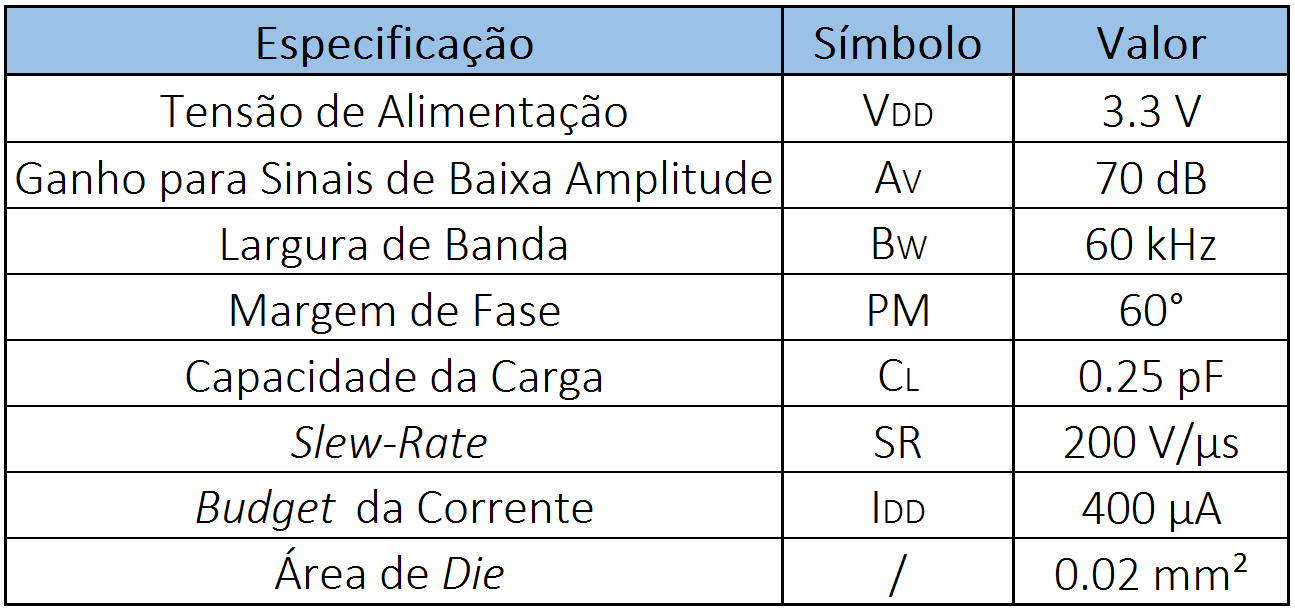
\includegraphics[keepaspectratio=true, scale=0.45]{teoricas/tabela1}
	\label{tab:tab1}
\end{table}

O circuito de ponto de partida para a realização do projecto é apresentado de seguida.

\begin{figure}[H]
	\centering
	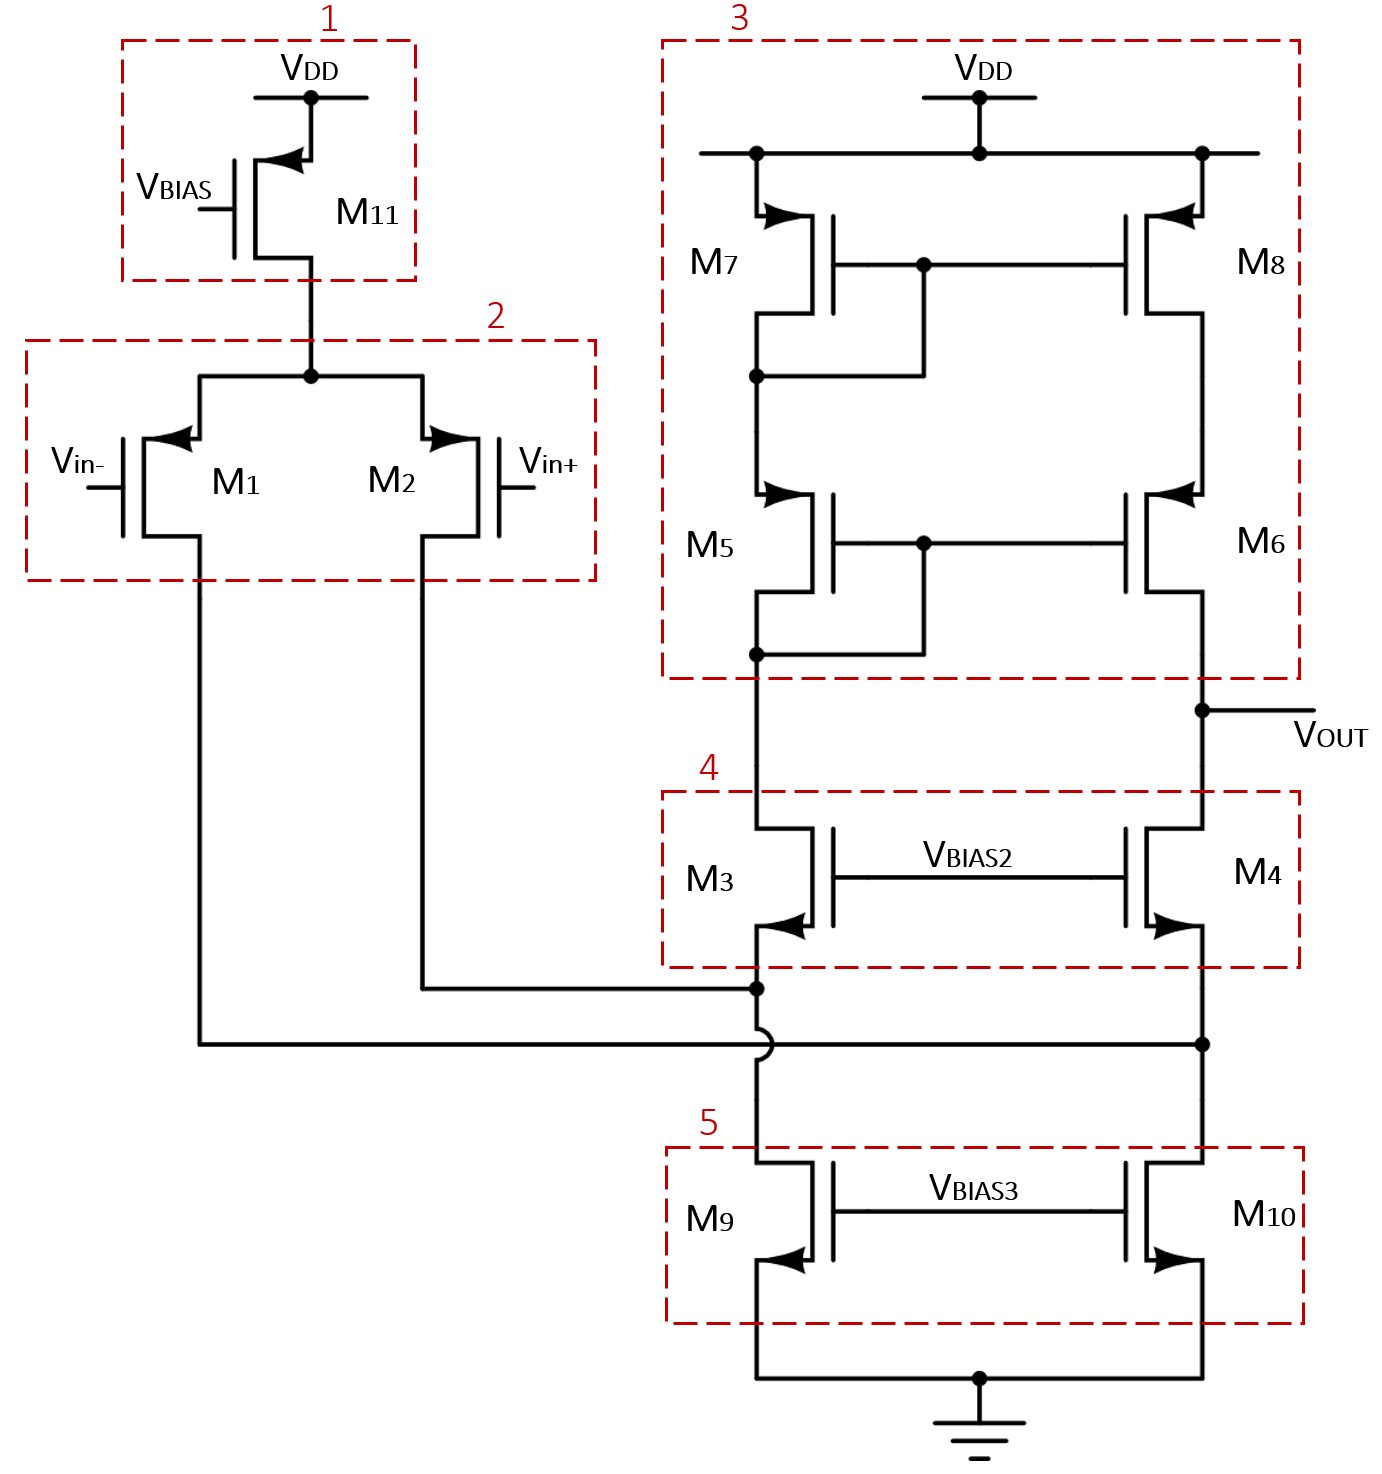
\includegraphics[keepaspectratio=true, scale=0.50]{teoricas/circuito1}
	\vspace{-0.5em}
	\caption{Circuito do amplificador a projectar.}
	\vspace{-0.8em}
\end{figure} 

\section{Adenda ao \textit{Middle Target}}

Esta secção foi acrescentada ao relatório final no intuito de corrigir os resultados obtidos e apresentados no relatório anterior, o do \textit{middle target}. Como referenciado, pretende-se projectar um amplificador \textit{folded cascode} CMOS OTA de dois andares de acordo com as especificações da Tabela \ref{tab:tab1}.

\subsection{Detecção dos erros} 

Foram identificados vários erros no relatório intermédio que comprometem os resultados apresentados anteriormente. A primeira correcção foi referente ao \textit{schematic} do \textit{testbench} que permite simular o circuito em testes de resposta AC. Foi colocado um \textit{switch} que simula a bobine - provoca um circuito aberto para um regime AC e curto-circuito para um regime DC. Foi também alterada a amplitude do sinal de entrada de 3.3 V para 1.6 V, sendo que esta alteração garante que os transístores não saem da saturação. De seguida pode-se comparar o novo \textit{testbench} com o anterior.

\begin{figure}[H]
	\centering
	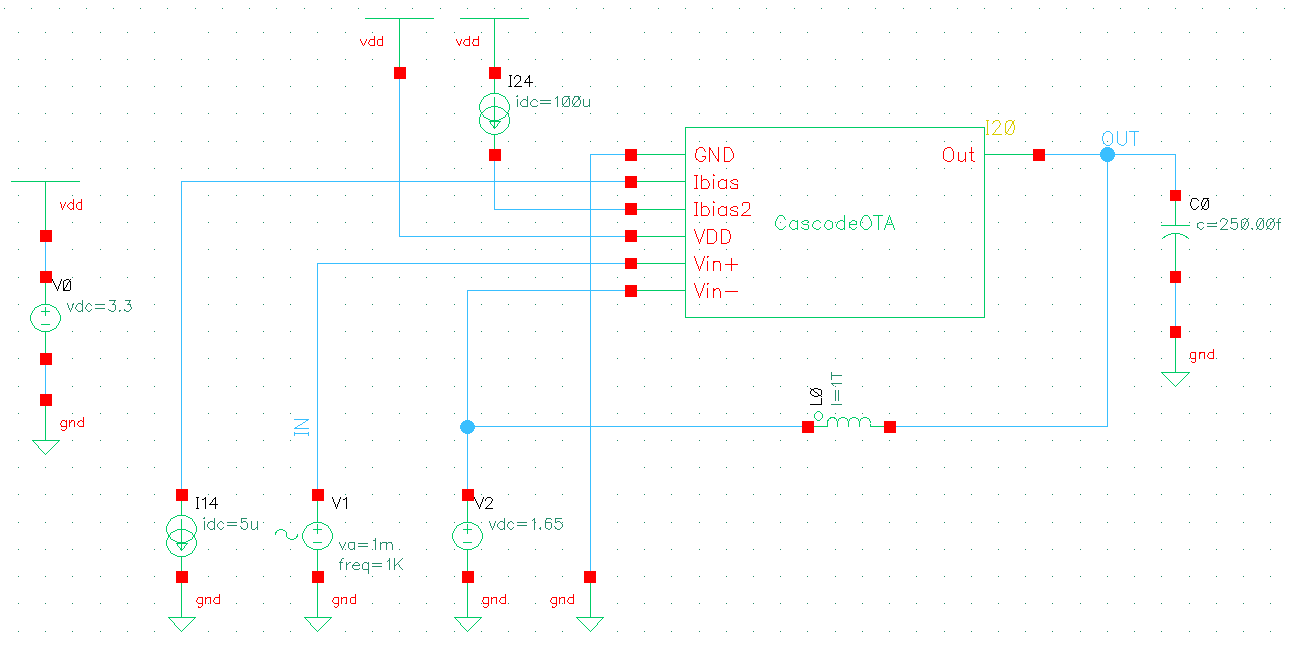
\includegraphics[keepaspectratio=true, scale=0.60]{exps/TBac}
	\vspace{-0.5em}
	\caption{\textit{Schematic} do \textit{testbench} anterior que permite simular o circuito em testes de resposta AC.}
	\vspace{-0.8em}
\end{figure} 

\begin{figure}[H]
	\centering
	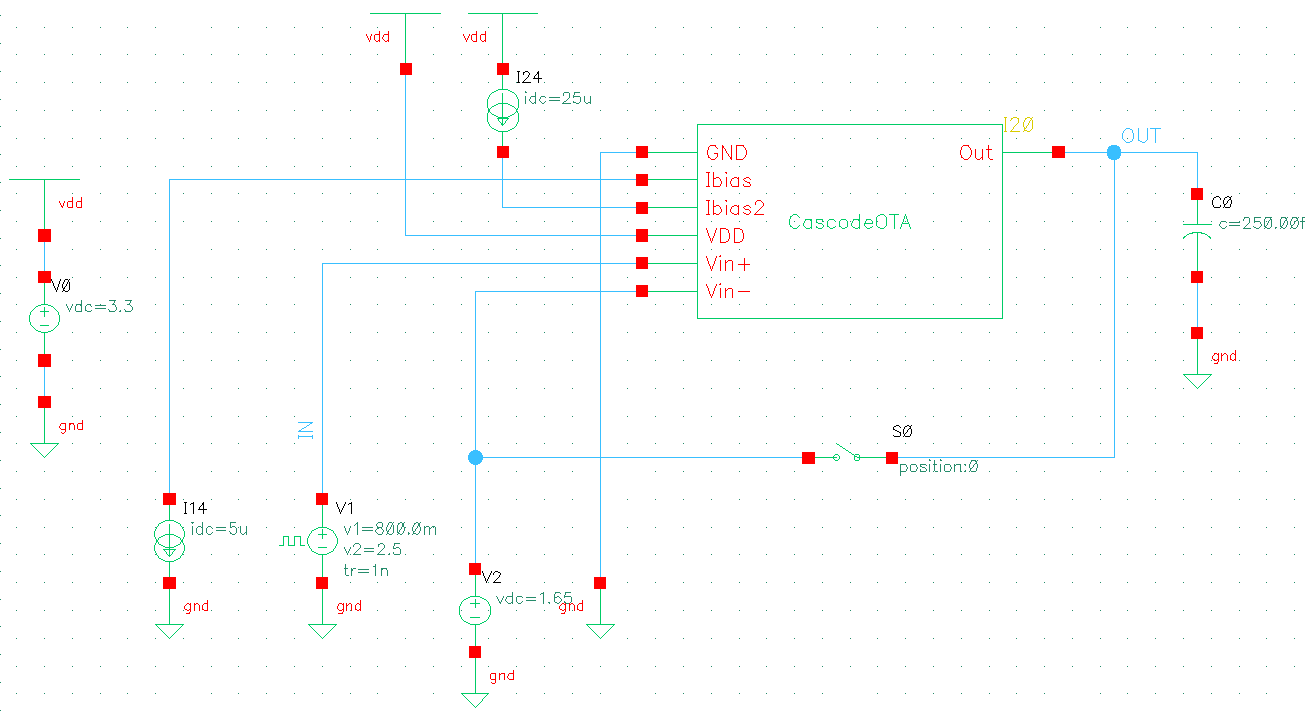
\includegraphics[keepaspectratio=true, scale=0.50]{exps/testebenchantigo}
	\vspace{-0.5em}
	\caption{\textit{Schematic} do novo \textit{testbench} que permite simular o circuito em testes da \textit{slew-rate} e de resposta transiente, DC e AC.}
	\vspace{-0.8em}
\end{figure} 

Outro erro identificado é referente ao cálculo da \textit{slew-rate}. No relatório intermédio, o resultado da \textit{slew-rate} era relativo só ao flanco de descida, sendo necessário demonstrar para os dois flancos - subida (equação 2.1) e descida (equação 1.2). 

\vspace{-3mm}
\begin{equation}
	\text{slewRate} (\text{VT("/OUT")} \:\: 1 \:\: \text{nil} \:\: 2 \:\: \text{nil} \:\: 10 \:\: 90 \:\: \text{nil} \:\: "\text{time}")
\end{equation}

\vspace{-3mm}
\begin{equation}
	\text{slewRate} (\text{VT("/OUT")} \:\: 2 \:\: \text{nil} \:\: 1 \:\: \text{nil} \:\: 10 \:\: 90 \:\: \text{nil} \:\: "\text{time}")
\end{equation}

\todo{falar destas expressoes - explicar das regioes de funcionamento dos transistores}

\todo{ha mais erros?}

\subsection{Correcção do dimensionamento}

\todo{explicar isto}

\info{nao esquecer que o racio de m1 e m2 mudou face ao da entrega intermedia, explciar porque}

Assim, o circuito final relativamente à entrega intermédia é:

\begin{figure}[H]
	\centering
	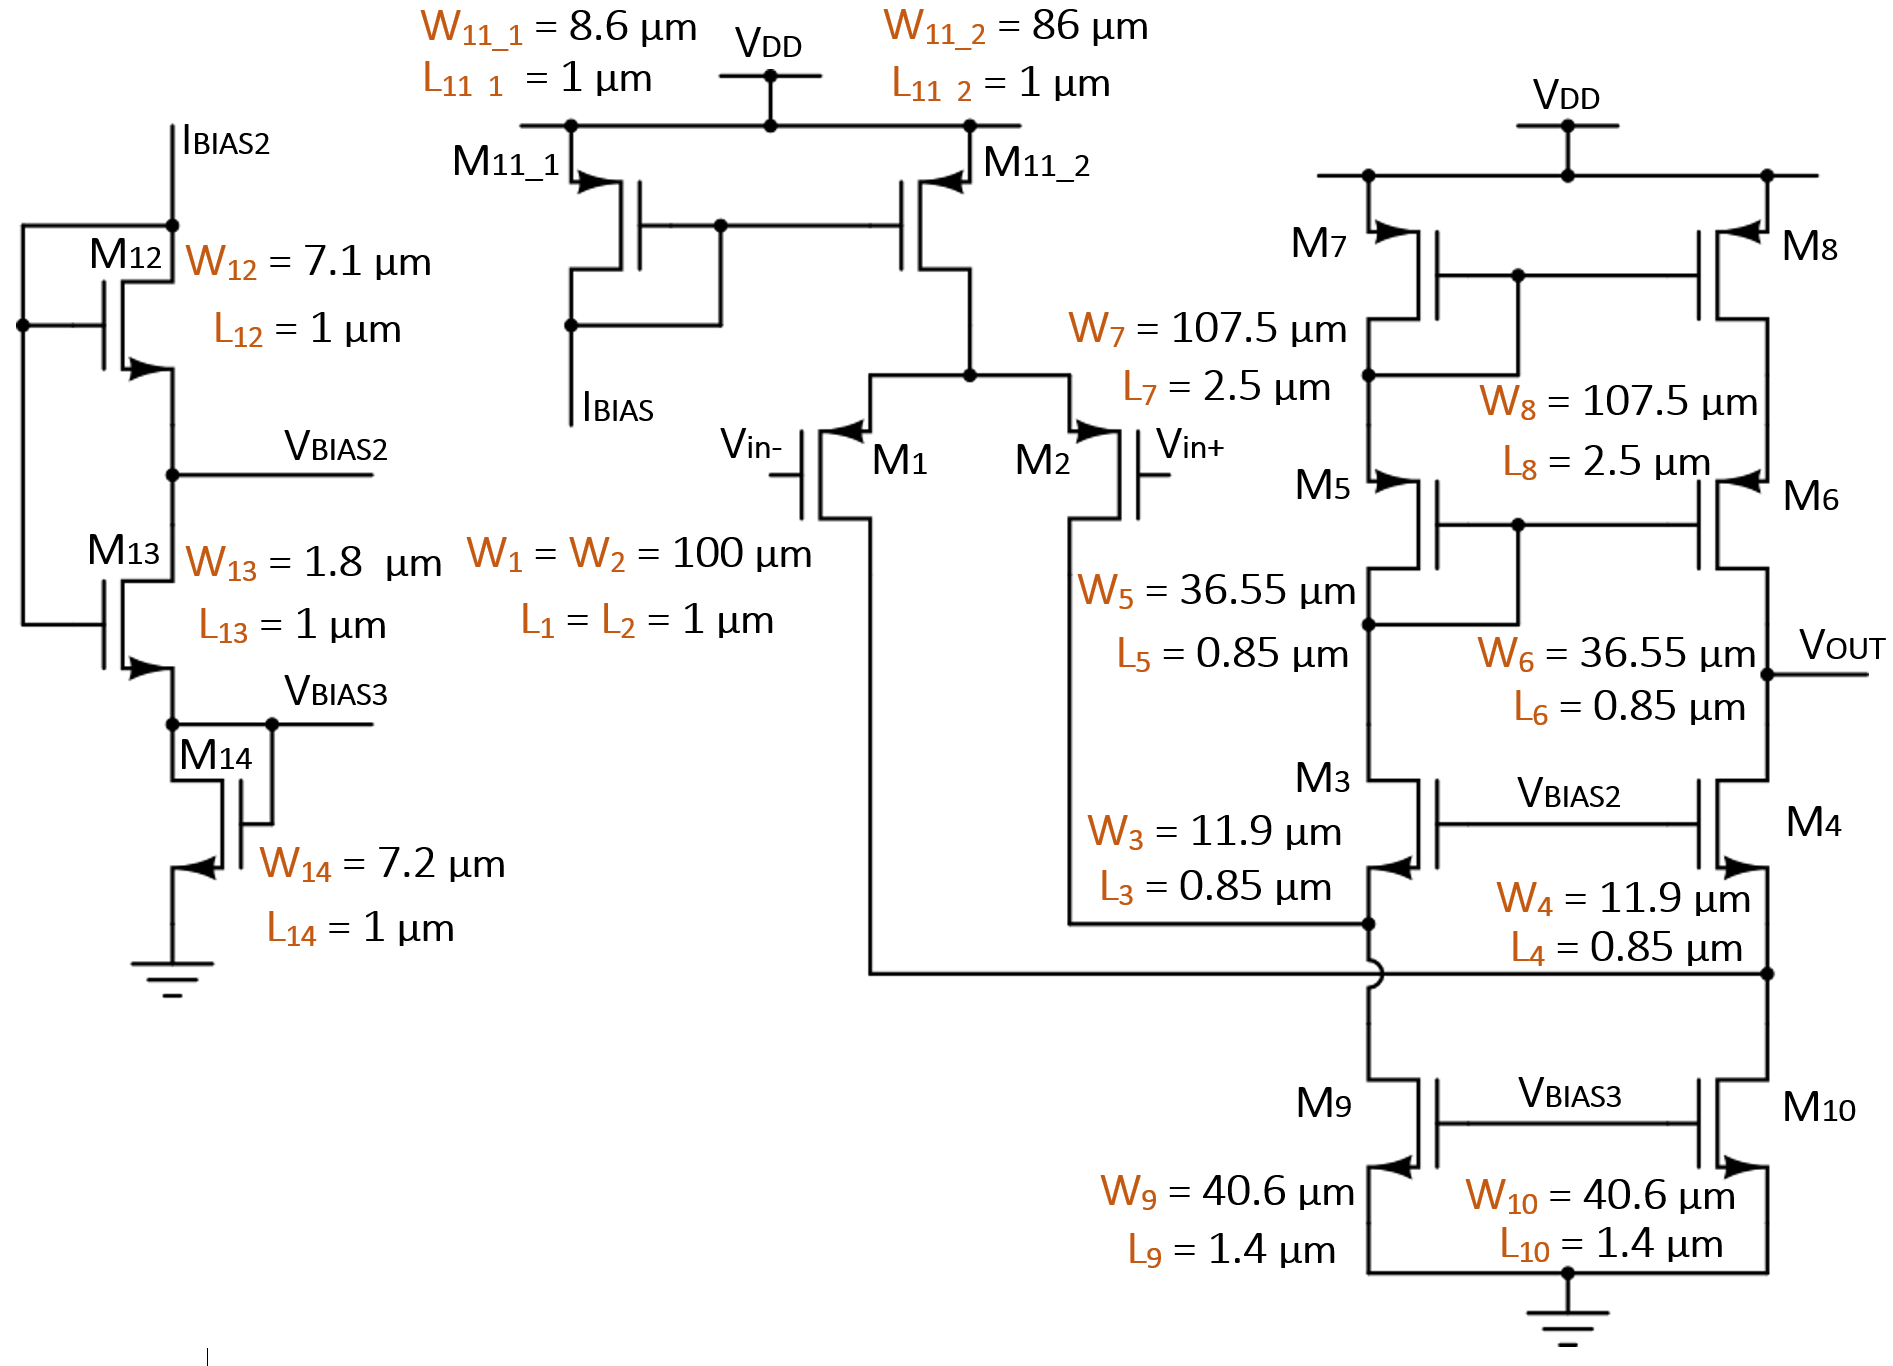
\includegraphics[keepaspectratio=true, scale=0.42]{teoricas/circuitoantesdadiv}
	\vspace{-0.5em}
	\caption{Circuito final da entrega intermédia.}
	\vspace{-0.8em}
	\label{fig:finalint}
\end{figure} 

\begin{table}[H]
	\centering
	\caption{Dimensões dos transístores que constituem o amplificador.}
	\vspace{-1.5mm}
	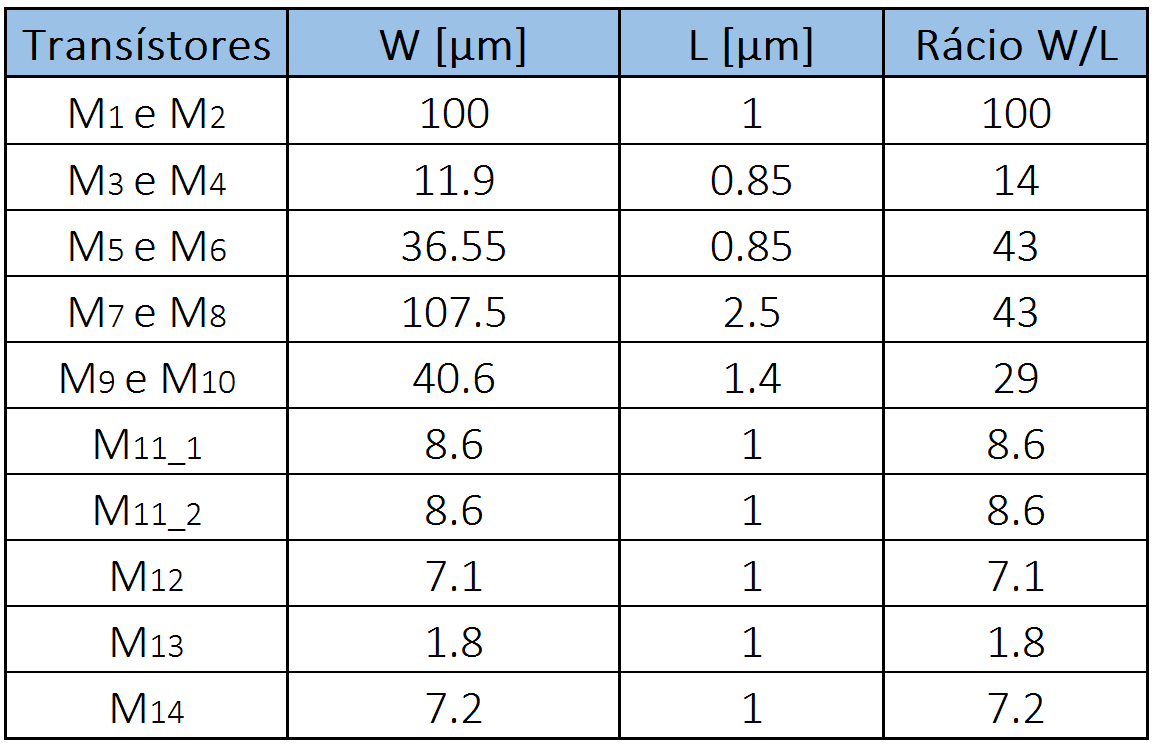
\includegraphics[keepaspectratio=true, scale=0.35]{teoricas/dimensoes1}
\end{table}

\subsection{Demonstração de resultados} 

Nesta secção apresenta-se os resultados do dimensionamento do relatório intermédio e do novo dimensionamento anteriormente referido, para simulações de Monte Carlo e de \textit{corners}.

\subsubsection{Resultados do dimensionamento inicial} 

\begin{figure}[H]
	\centering
	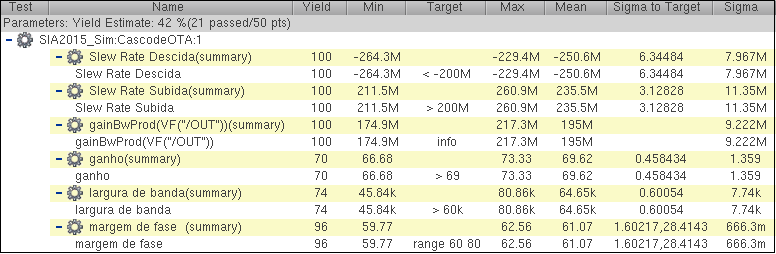
\includegraphics[keepaspectratio=true, scale=0.65]{exps/MonteCarlo_50pt_Antigo}
	\vspace{-0.5em}
	\caption{Simulação de Monte Carlo para 50 pontos.}
	\vspace{-0.8em}
\end{figure} 

\begin{figure}[H]
	\centering
	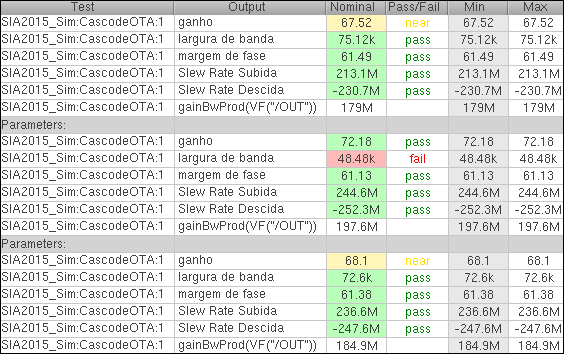
\includegraphics[keepaspectratio=true, scale=0.65]{exps/MonteCarlo_3pt_Antigo}
	\vspace{-0.5em}
	\caption{Resultados obtidos para as 3 primeiras simulações de Monte Carlo.}
	\vspace{-0.8em}
\end{figure} 

\begin{figure}[H]
	\centering
	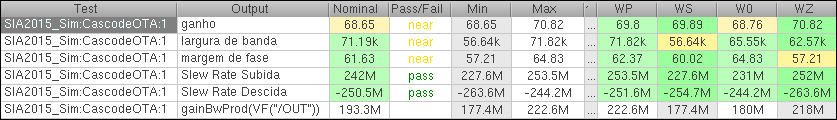
\includegraphics[keepaspectratio=true, scale=0.65]{exps/Corners_Antigo}
	\vspace{-0.5em}
	\caption{Simulação por \textit{corners}.}
	\vspace{-0.8em}
\end{figure} 

\subsubsection{Resultados do dimensionamento corrigido} 

\begin{figure}[H]
	\centering
	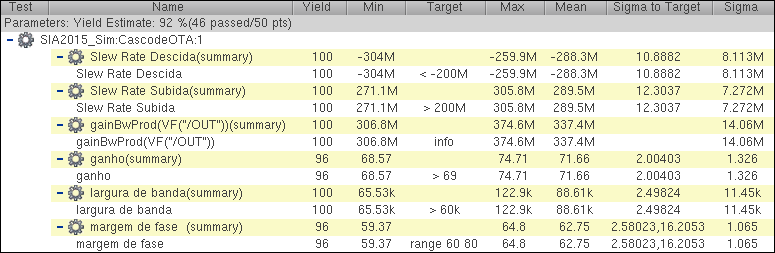
\includegraphics[keepaspectratio=true, scale=0.65]{exps/MonteCarlo_50pt_Novo}
	\vspace{-0.5em}
	\caption{Simulação de Monte Carlo para 50 pontos.}
	\vspace{-0.8em}
\end{figure} 

\begin{figure}[H]
	\centering
	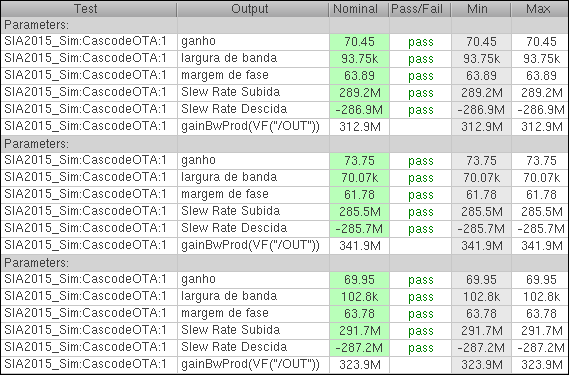
\includegraphics[keepaspectratio=true, scale=0.65]{exps/MonteCarlo_3pt_Novo}
	\vspace{-0.5em}
	\caption{Resultados obtidos para as 3 primeiras simulações de Monte Carlo.}
	\vspace{-0.8em}
\end{figure} 

\begin{figure}[H]
	\centering
	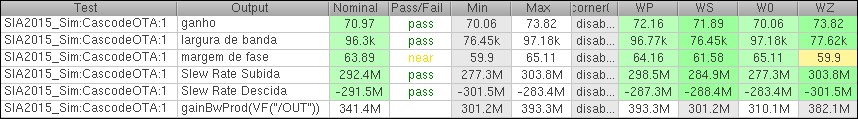
\includegraphics[keepaspectratio=true, scale=0.65]{exps/Corners_Novo_semDiv}
	\vspace{-0.5em}
	\caption{Simulação por \textit{corners}.}
	\vspace{-0.8em}
\end{figure} 

\todo{comentar diferenças obtidas}

\section{Projecção do \textit{Layout}}

\subsection{Multiplicidade e \textit{Fingers}}

Para projectar o \textit{layout} do circuito da Figura \ref{fig:finalint} optou-se por dividir os transístores de grandes dimensões com recurso a duas técnicas - multiplicidade e \textit{fingers}. A técnica de \textit{fingers} corresponde a um arranjo específico do transístor com $n$ \textit{gate fingers} em que as difusões da \textit{source} e do \textit{drain} são partilhadas. Se se tiver $n$ \textit{fingers} haverá então $n+1$ difusões. A multiplicidade é quando se faz uma ligação em paralelo de múltiplos dispositivos MOS, sendo que o agregado deles corresponde a um só transístor. 

Do ponto de vista da definição correspondem ao mesmo, mas são de facto duas maneiras diferentes de pensar na paralelização de transístores. Com o recurso a \textit{fingers} tem-se uma única célula com o transístor completo com todos os \textit{fingers}, útil para quando se quer uma célula mais compacta, enquanto na multiplicidade tem-se tantos transístores quanto a multiplicidade indicar. De facto, é possível conjugar as duas técnicas, ou seja, cada dispositivo MOS da multiplicidade pode ser feito com vários \textit{fingers}.

\todo{criterio para as multiplicidades e fingers do transistores}

Assim, na tabela seguinte encontra-se uma descrição de como são constituídos os vários transístores do circuito.

\begin{table}[H]
	\centering
	\caption{Dimensões e características dos transístores do amplificador.}
	\vspace{-1.5mm}
	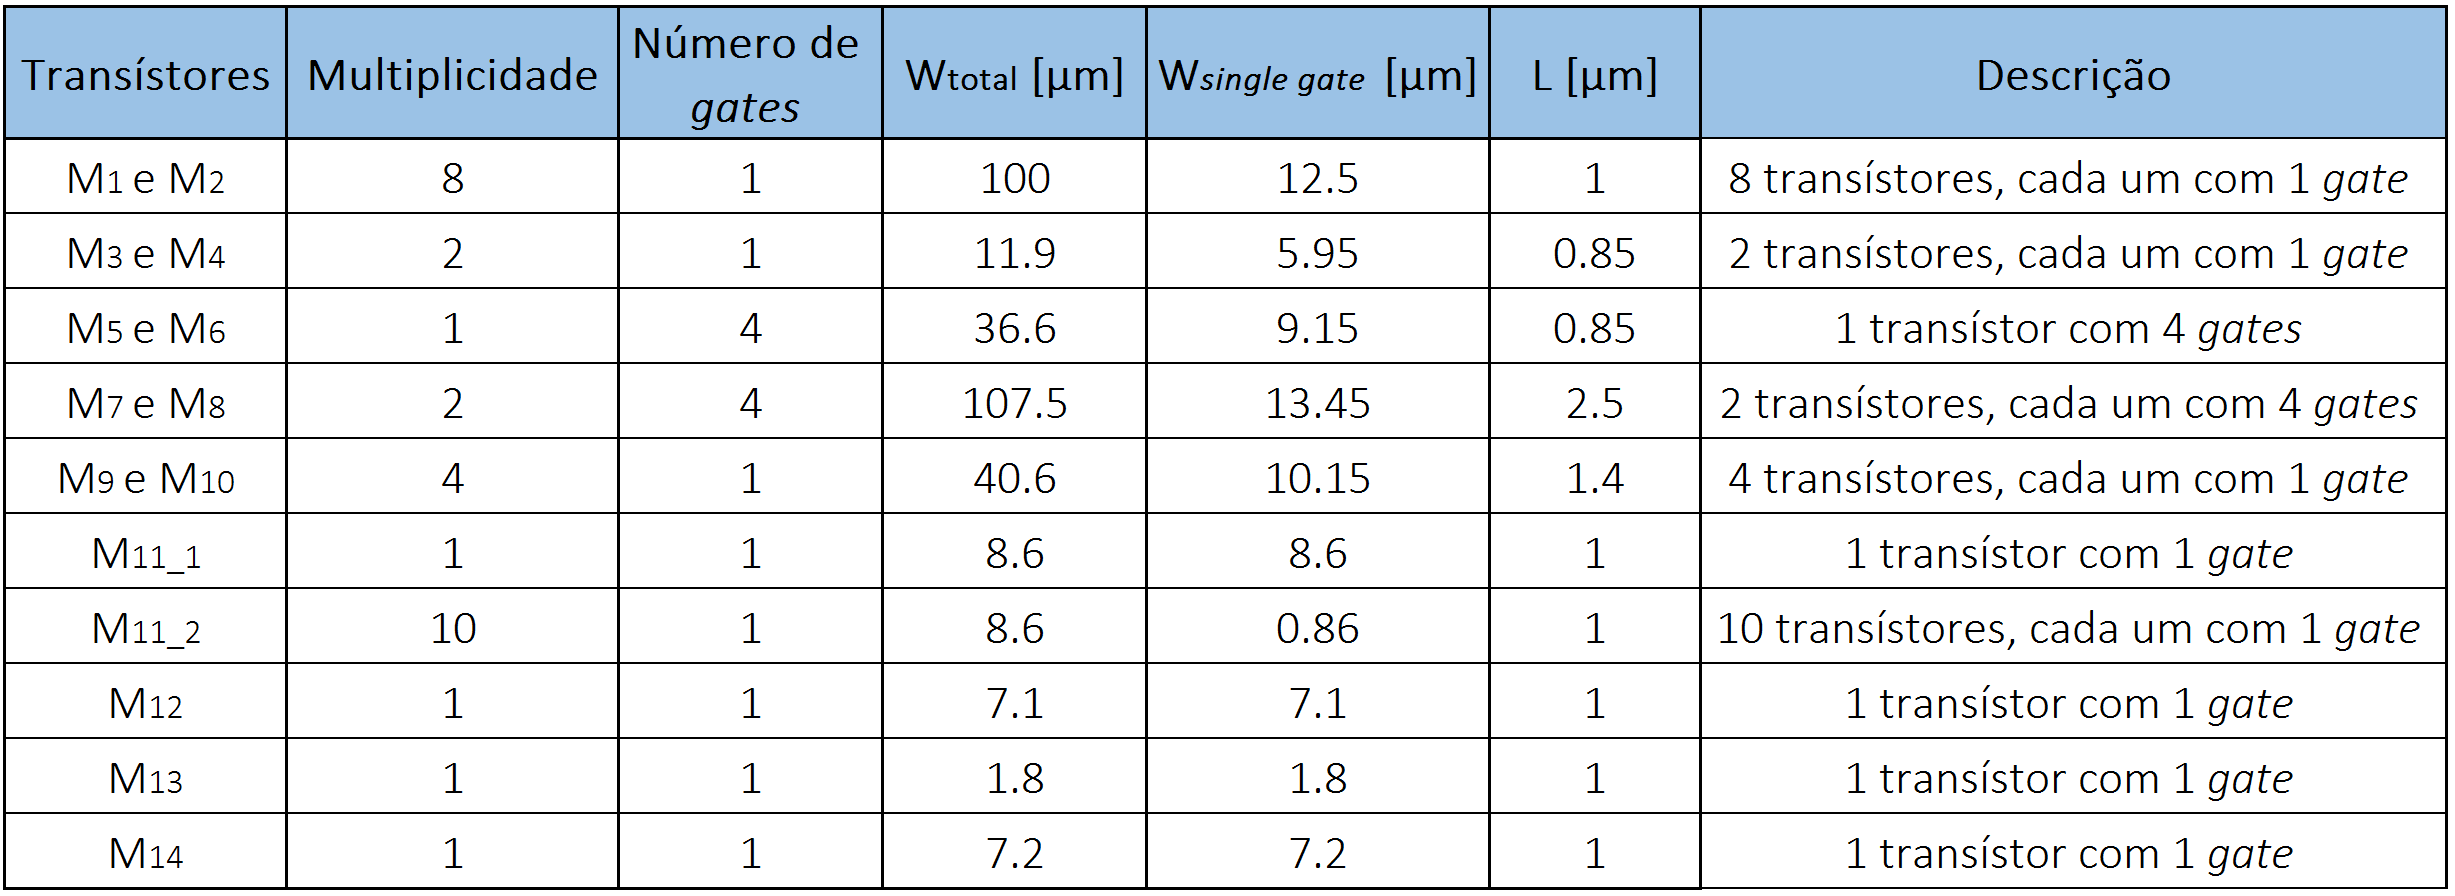
\includegraphics[keepaspectratio=true, scale=0.30]{teoricas/dimensoes2}
\end{table}

\subsection{Disposição dos transístores}

Depois de se definir como estão estruturados os vários transístores é importante definir como se encontram dispostos no \textit{layout}. A topologia básica que foi utilizada é a de \textit{common centroid}. Através desta técnica consegue-se garantir um melhor \textit{matching} entre dois transístores iguais e em que se pretende um comportamento semelhante. De facto, o \textit{common centroid} é utilizado para se garantir que, e.g., um amplificador diferencial tenha um sinal de modo comum próximo de 0 e, como tal, um CMRR maior.

Para o circuito em causa foram definidos 4 blocos principais sobre os quais se definiu uma estrutura \textit{common centroid}:

\begin{itemize}
	\item espelho de corrente básico que é polarizado em corrente com $I_{BIAS}$ (equivalente ao Bloco 1 da Figura 1);
	\vspace{-2mm}
	\item transístores do par diferencial (Bloco 2 da Figura 1);
	\vspace{-2mm}
	\item espelho de corrente cascode básico do tipo PMOS (Bloco 3 da Figura 1);
	\vspace{-2mm}
	\item transístores do tipo NMOS.
\end{itemize}

\pagebreak

\section{Conclusões}

\end{document}